\subsection{Hardware}
In this section we introduce the hardware setup we created in order to validate our chip design. 
Our goal is to reproduce the same tests with the produced chip as we used to validate the design in the simulation. We therefore tried to create hardware that replicates the virtual test bench setup as close as possible. Of particular interest to us are dynamic regulation characteristics of the buck-boost converter, as they give insight into the closed loop regulation characteristics like bandwidth and phase margin. In addition we want to test the functionality of the SPI interface as well as have the ability to measure internal signals such as the internal clock oscillator and the the band gap reference voltage. \\
List of measurements:
\begin{itemize}
    \item Line regulation
    \item Load regulation
    \item Output voltage regulation accuracy 
    \item Efficiency
    \item Startup behavior
    \item Short circuit behavior
    \item SPI functionality
    \item Clock frequency
    \item Band gap reference voltage
\end{itemize}

Going further with the test bench analogy, we split the test setup into two components, a test bench like PCB with call the Adapter PCB and multiple smaller PCBs which contain the \ac{DUT}, we refer to as Hats.


\subsubsection{Adapter PCB}
The main Adapter PCB contains the functionality of the test bench and has a common plug-in location for the \ac{DUT} containing Hats. The Adapter is designed in such a way, that the \ac{DUT} can be placed in the thermal chamber of the thermal airstream system TP04300A in order to test the \ac{DUT} functionality under various thermal conditions. The PCB contains four electronically controllable loads for load step measurements and contains current sense amplifiers to measure the current flowing in and out of the switching converter on the \ac{DUT}. To test the SPI communication with the \ac{DUT} we have included an Arduino Every Nano which allows us to use easily create a program to read and write to registers on the \ac{DUT}.

\begin{figure}[h]
    \centering
    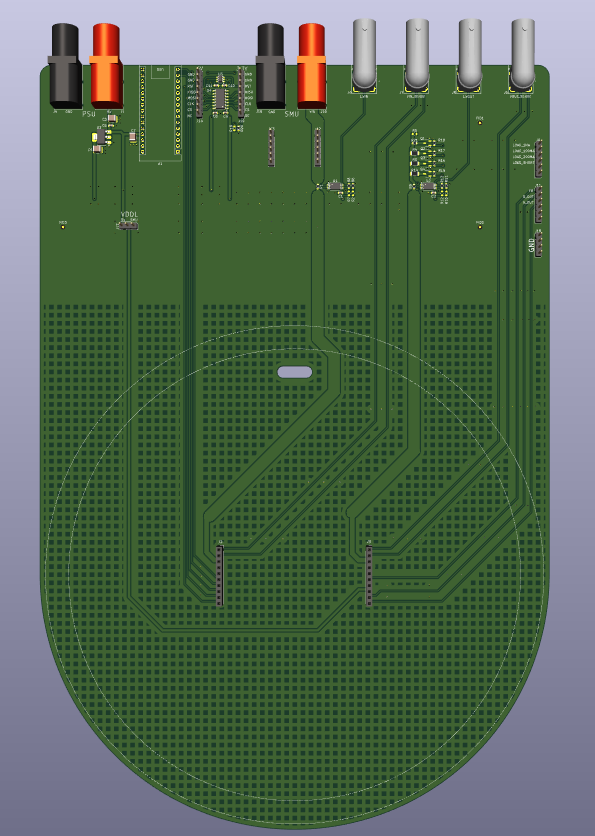
\includegraphics[width=0.8\textwidth]{../ASIC-DESIGN-2/images/02_test_setup/Adapter _PCB.png}
    \caption{3D render of the Adapter PCB}
    \label{fig:Adapter_PCB}
\end{figure}



\subsubsection{Hat PCB}
In total we created three Hat PCBs which can be used as \ac{DUT}s. One PCB contains a commercially available IC and we created to PCBs for our manufactured chip. In the first PCB our chip is socketed and in the second one we soldered the QFN package to the board. The socketed version allows for the quick characterization of multiple chips and measurement of the variance of characteristics over the batch. The socket however introduces higher lead resistances and inductances as well as thermaly isolates the chip from the PCB. The thermal isolation could lead to increased temperatures in high load conditions and in the worst case could lead to damge of the chip. We do not expect these factors to play a major role for the characteristics we want to measure, but out of caution we decided still to create a PCB with the chip directly soldered to the PCB. This allows us to verify our assumption and gives us a fallback, if our assumption turns out to be false and chip does not function correctly when socketed. \\

\begin{figure}[h]
    \centering
    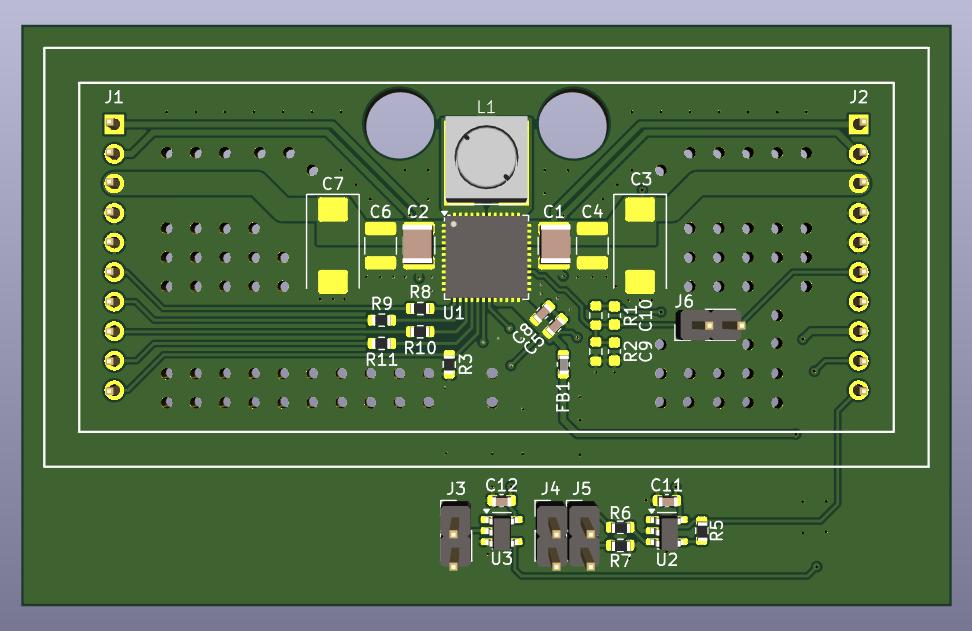
\includegraphics[width=0.8\textwidth]{../ASIC-DESIGN-2/images/02_test_setup/ASIC_Hat_PCB.png}
    \caption{3D render of the Hat PCB with the QFN package soldered to the PCB}
    \label{fig:ASIC_Hat}
\end{figure}


Our reasoning to create a Hat with a commercially available chip is two fold. First it allows us to test our test setup with a real hardware \ac{DUT} before we receive our fabricated chip and also gives us a baseline to compare our chip against. For the commercially available IC we decided to use the TPS63900 from Texas Instruments. While this IC is significantly smaller in size it has a similar input and voltage range as well as current drive capabilities. It is also a highly integrated buck-boost converter with integrated switches in the standard cascaded-buck-boost converter topology. 

